% ================================================================
% ================================================================
% --- PREAMBLE
% --- Document class
\documentclass[12pt]{article}

% --- Packages
\usepackage[utf8]{inputenc}
\usepackage[top=1in, bottom=1in, left=1in, right=1in]{geometry}
\usepackage{setspace}
\usepackage{microtype}
\usepackage[dvipsnames]{xcolor}
\usepackage{lastpage}
\usepackage{hyperref}
\usepackage{fancyhdr}
\usepackage{booktabs}
\usepackage{graphicx}
\usepackage{todonotes}
\usepackage{fontspec}
\usepackage{adjustbox}
\usepackage{float}
\usepackage{dcolumn}
\usepackage[backend=biber, style=apa, citestyle=apa]{biblatex}

% --- Settings
%\setmainfont{Caladea}
\usepackage{libertine}
\usepackage[libertine]{newtxmath}
\addbibresource{references.bib}

\hypersetup{
    colorlinks = true,
    linkcolor  = blue,
    urlcolor   = blue,
    citecolor  = blue,
    }
    
\pagestyle{fancy}

% --- Header and footer
\fancyhf{}
\headheight = 28pt
\chead{20 YEARS OF DOLLARIZATION IN ECUADOR\\
       \textit{Nicolás Cachanosky and John Ramseur}}
\cfoot{\footnotesize Page \thepage \hspace{0.5pt} of \pageref{LastPage}} 

% --- Title page
\title{20 YEARS OF DOLLARIZATION IN ECUADOR: A SYNTHETIC CONTROL ANALYSIS
       \thanks{We appreciate comments by Lawrence H. White. Any error or omission is our own.} \\
       \bigskip}

\author{
        \textbf{Nicolás Cachanosky} \\
        Metropolitan State University of Denver \\
        Department of Economics \\
        \href{mailto:ncachano@msudenver.edu}{ncachano@msudenver.edu} \\
        \and
        \textbf{John Ramseur} \\
        Metrpolitan State University of Denver \\
        Department of Economics \\
        \href{mailto:jramseur@msudenver.edu}{jramseur@msudenver.edu} \\
        \bigskip}

\date{\today}


% ================================================================
% ================================================================
% --- DOCUMENT
\setlength{\marginparwidth}{2cm}
\begin{document}


% ================================================================
% --- TITLE PAGE

\maketitle

\begin{abstract}
\noindent
This paper uses a Synthetic Control Analysis to examine the economic effectiveness of dollarization in Ecuador. We address common concerns surrounding the adoption of dollarization as a policy and provide several solutions to those concerns. We find that dollarization resulted in significant higher levels of income without clear evidence of worsening in social health variables such as infant mortality, poverty, and income distribution.
\end{abstract}

\bigskip \bigskip
\footnotesize \noindent \textbf{JEL codes}: E42; E50; O43 \\
\footnotesize \noindent \textbf{Keywords}: Ecuador, dollarization, synthetic control analysis

\newpage
\doublespacing


% ================================================================
% --- SECTION 1: INTRODUCTION
\section{Introduction} 
    \label{sec:intro}

The issue of dollarization was a topic of debate at the turn of the century because of a series of financial crisis in emerging economies. Besides the international crises of the late 1990s, some countries faced their own issues. Ecuador dollarized its economy after an inflation crisis. Argentina's currency board was abandoned in 2001, triggering one of its largest economic crisis since its independence. El Salvador dollarized its economy in 2001.

Even though history offers more than hundred cases of dollarization \parencite{Schuler2005}, usable data for typical regression analysis remains limited. Maybe this is a reason why the discussion surrounding dollarization has remained highly speculative \parencite[for a sample see][]{Levy-Yeyati2002,Salvatore2003}. However, twenty years of dollarization in Ecuador offer an informative case study for other economies with troubled currencies, such as Argentina or Venezuela. 

Previous work on Ecuador's dollarization looks at issues such as the loss of seigniorage \parencite{Lange2005}, its effects on fiscal policy \parencite{MariDelCristo2016}, or how feasible it is to de-dollarize Ecuador \parencite{JAMESON2003}. In addition, Jansen and Ortiz \parencite*{Jansen2007} find that the probability of large negative returns in stocks decreased post dollarization while that of positive returns increased.

This paper offers the Nobel application of a synthetic control analysis (SCA) \parencite{Abadie,Abadie2003,Abadie2015} to the case of Ecuador's dollarization. This method builds a synthetic non-dollarized Ecuador that can be used as a counterfactual of its dollarization in 2001. We find that dollarized Ecuador outperforms the synthetic non-dollarized Ecuador in variables such as real GDP per capita, unemployment, and income distribution. We also find inconclusive results in changes to total factor productivity (TFP). The ideal counterfactual to evaluate the effects of dollarization in Ecuador is not to compare economic variables before and after dollarization, but to compare dollarized Ecuador with a non-dollarized Ecuador. SCA is useful because a real-world non-dollarized Ecuador is not observable.\footnote{In recent years, SCA has been applied in a number of different studies. For instance, Rok \parencite*{Spruk2019} studies the economic cost of institutional shocks to Argentina; Grier and Maynard \parencite*{Grier2016} and Absher, Grier, and Grier \parencite*{Absher2020} study market reforms in Georgia; and Powell, Clark, and Nowrasteh \parencite*{Powell2017} look at the impact of mass immigration in Israel.}

Some scholars consider dollarization to be a good (or second best) reform for countries with troubled currencies \parencite{Avila2019,Cochrane2018,Gale2002,Hanke2003a,White2014a}. Other scholars are critical of dollarization; Sachs and Larrain \parencite*{Sachs1999} offer a good representation of those who oppose to dollarization arguing that it is a "reckless" (p. 80) straitjacket. 

The paper proceeds in the following way. Section 2 reviews how typical functions of a well-functioning central bank such as being a lender of last resort (LOLR) or domestic monetary policy can be replaced under dollarization. Section 3 presents the SCA analysis and results. Section 4 concludes.


% ================================================================
% --- SECTION 2: HOW CAN DOLLARIZATION REPLACE TYPICAL ROLES OF A CENTRAL BANK
\section{How can Dollarization Replace Typical Roles of a Central Bank}
    \label{sec:debate}

Dollarization is the adoption of a foreign currency by a domestic country whether the currency adopted is the US dollar (USD), the New Zealand dollar, the Euro, the British Pound, or any other foreign currency. Dollarization can either by unilateral or bilateral. In the former case, the dollarizing country unilaterally decides to adopt a foreign currency. In the latter, there is an agreement with the central bank that can include, for instance, sharing some of the new seigniorage that dollarization will bring.

Another issue to consider is that dollarization can also be either formal or informal. In the former case, the government formally adopts a foreign currency, while in the latter case economic agents decide to use a foreign currency regardless of the government's mandate. The distinction between formal and informal dollarization is important because it draws a distinction between a spontaneous and planned dollarization reforms. In the first case we have a bottom-up institutional change spontaneously driven by the private sector. In the second case we have a top-down government reform. Ecuador represents a bottom-up dollarization in the sense that it was the public who chose to use the USD and later on the government decided to formalize such decision \parencite{White2014a}. It was not the government who imposed the USD on the public, it was the public who imposed the USD on the government.\footnote{For a more detailed analysis if Ecuador's dollarization see Beckerman and Solimano \parencite*{Beckerman2002}.} An example of an informal dollarized economy is Argentina, where the public saves and demands USDs, but the government maintains the peso in circulation.

The idea of dollarization can be split in two. The \textit{naive} view assumes that dollarization is \textit{sufficient} reform to get back the economy on track. On the other hand, the \textit{savvy} view takes the position that dollarization is a \textit{necessary} (even if not sufficient) reform needed to get the economy back on track. The naive version is a straw-man version of the savvy view and, therefore, the wrong target of criticism. 

Dollarization is seen to produce at least three problems: (1) the loss of domestic monetary policy, (2) the absence of a lender of last resort (LOLR), and (3) the loss of seigniorage. There is a fourth issue. Because savvy dollarization requires other reforms such as a balanced budget, it seems that dollarization becomes unnecessary by its necessary conditions. We discuss these four issues next.

% --- SUB-SECTION 2.1
\subsection{The Problem of Loosing Monetary Policy}

When a country dollarizes it gives up the possibility of executing its own domestic monetary policy. The possibility of executing monetary policy is particularly important in the case of foreign nominal shocks that would require a prudent and well calibrated reaction by a domestic central banks. Yet, the point of dollarization is precisely to eliminate domestic policy. The reason is that domestic policy proves to be worse than being exposed to foreign nominal shocks. The domestic central bank because its a constant source of nominal shocks and high inflation rather than a source of monetary stability. It is important to keep in mind that dollarization is an issue in countries with extreme or long-lasting monetary imbalances. These are countries where a well-functioning and independent central bank is unfeasible.

A cost-benefit analysis of dollarization must avoid falling into the Nirvana fallacy \parencite{Demsetz1969}. The opportunity cost of dollarization is not a well-functioning central bank, it is the chronically inefficient monetary policy affecting the country. Countries that face a potential dollarization do not have ideal central banks, they have very inefficient ones. The realistic choice is between dollarization and a central bank unable to commit to efficiency.

It is also unclear that in countries that face a potential dollarization domestic monetary policy is as independent as it is assumed to be. A detachment from foreign nominal shocks requires the adoption of a free floating exchange rate. However, many developing countries suffer from feat of floating \parencite{Calvo2002}, which means that in practice the domestic central bank is deviating from the ideal domestic strategy and, to some extent, following foreign monetary policy. If domestic monetary policy is going to be reticent to devalue or appreciate when facing foreign shocks, then it is unclear what benefit the domestic country is giving up by dollarizing. In other words, the alleged benefit of a domestic central bank is inversely related with the degree of fear of floating.\footnote{Levy-Yeyati, Sturzenegger, and Gluzmann \parencite{Levy-Yeyati2003} argue that some countries face more fear of appreciation than of depreciation.}

For the purpose of framing the discussion, assume the domestic central bank follows the following Taylor-rule reaction function.\footnote{This policy reaction is presented just for illustration purposes. A country that faces a potential dollarization is in such monetary disorder that the central bank may not follow any reaction policy other than a day-to-day decision about how to make it to the next day.}

\begin{equation} \label{Eq:1}
    i_t = i^*_t + \phi_\pi \tilde{\pi}_t + \phi_X \tilde{X}_t + \varepsilon_t
\end{equation}

where $t$ is the time period, $i$ and $i^*$ denote short-term and short-term equilibrium interest rates respectively, $\tilde{\pi}$ is the inflation gap, $\tilde{X}$ is the gap of other feedback variables (such as output or unemployment gap), $\phi$ are positive numbers and $\varepsilon$ is an error term or shock.

A deviation form the interest rate dictated by the policy rule would produce economic costs, such a deviation from the inflation target, misallocation of resources, relative price distortion, monetary illusion, and so on. Yet, large negative shock (a large negative $\varepsilon$) can originate externally and also domestically. Far from being a settled issue, comparing the costs of domestic and external monetary shocks is an empirical question.

Consider the case of Ecuador itself, between 1983 and its dollarization in 2000, the average yearly inflation rate was 42.2-percent. In terms of external large nominal shocks, Ecuador did not only faced the 2008 crisis, it also declared a default on its sovereign debt. Instead of falling into a large crisis, as would be expected from a shock as significant as the 2008 crisis, real GDP per capita fell just 1.1-percent in 2009 starting to grow again next year. In comparison, Argentina's real GDP fell 6.9-percent in 2009 despite not being dollarized and having its own central bank. Consider now a source of domestic nominal shocks. Between the rise of Perón in 1946 and 2020, the yearly average inflation rate in Argentina is 62-percent. It is not clear that 74 years of an average inflation rate of 62-percent (which is also highly volatile) is better than monetary stability through dollarization.


% --- SUB-SECTION 2.2
\subsection{The Problem of the Absence of a Lender of Last Resort}

A dollarized economy does not have a central bank to perform the duties of a LOLR. This is problematic because the financial market is seen as inherently unstable. According to this view, illiquid banks are prone to suffer a bank run. If the bank run spreads through the financial market, then a LOLR is needed to get the situation under control and avoid a major financial crisis. For the purpose of this paper, we take the inherent instability of the banking sector as given.\footnote{The inherent instability view of banks rests on the Diamond and Dybvig \parencite*{Diamond1983} model. For a critical review of this model and its implications see Cachanosky \parencite*[][Ch. 1]{Cachanosky2018a}, Dowd \parencite*{Dowd1992a}, Selgin \parencite*[][Ch. 11]{Selgin1996c}, and White \parencite*[][Ch. 6]{White1999c}.}

Using Bagehot's rule as reference, a LOLR should lend only at a premium rate only to illiquid but solvent banks. A central bank can deviate from this rule, which leads to moral hazard problems. As long commercial banks expect the central bank to offer bailout to insolvent banks, then said banks will be inclined to invest in riskier assets increasing the likelihood of a financial crisis. To avoid moral hazard, a central banks adherence to Bagehot's rule must be credible. This is not easy because central banks can bailout as many banks as desired without suffering losses or going bankrupt. In these terms, dollarization can be seen as a credible commitment to not bailout banks at the cost of not being able to do so when needed \parencite{Gale2002}. The credibility reading of dollarization is relevant for countries where central banks presidents do not face incentives to increase credibility due to their short term in office.\footnote{For instance, the Argentine central bank had 23 presidents between 1983 and 2015, with an average of 570 days in office.}

However, a central bank is no the only form of a LOLR. Therefore, dollarization does not mean there will be no LOLR, it means this role will not be performed by the domestic monetary authority. One alternative to the central bank as a LOLR is what Ecuador does, which is having a special tax on deposits to fund a liquidity fund that can be used if needed by a designated institution \parencite{Quispe-Agnoli2006}. This fund can be managed by a public office (as is the case of Ecuador) or by a consortium of private banks, who face the incentive to bailout only solvent banks. Another options is to mandate a deposit insurance.\footnote{The case of the United States is telling. Bank failures decreased with the implementation of the FDIC, not with the establishment of the Federal Reserve in 1913. See Selgin, Lastrapes, and White \parencite*[][pp. 582-583]{Selgin2012a}.} A third case would be to allow a deep financial integration with international markets. This is the case of Panamá \parencite{MorenoVillalaz1999,MorenoVillalaz2005}. Banks operating domestically can be owned by foreign banks, who would have the motivation and information to keep their international branches in a good financial situation. There is also the option of regulating reserve requirements and credit diversification. In short, the option is not between a LOLR (central bank) and no LOLR (dollarization). A range of different version of a LOLR are available. What is needed is an entity able to lend, not necessary one that can "print" its own money \parencite{Calvo2001}.

In addition, the capacity of a domestic central bank who serves as LOLR should not be overstated. Countries that face a potential dollarization do not have a high demand of their domestic currency. The run is not against banks, it is against the domestic currency (which happens to be deposited in banks). The domestic central bank cannot "print" USD, and therefore there is only so much it can do to stop a bank run. The pesos supplied by the domestic central bank find their way to the exchange rate market. Absent strict capital controls to the domestic private sector, the supply of pesos fuels a currency crisis.

The more private-market oriented a LOLR is, the closer it will adhere to Bagehot's rule minimizing moral hazard. A privately managed fund risks facing loses if it saves banks that are insolvent, but a central bank doe not face the same cost-benefit incentives. The underlying issue in the case of dollarization is not whether or not to have a LOLR, but what type of LOLR should be in place. One that operates under the scope of government incentives, or one that operates under the scope of market incentives.\footnote{Bagehot's rule was endorsed by Ben Bernanke when serving as Chairman of the Federal Reserve. It is less clear that the acts of the Fed followed this endorsement \parencite{Hogan2015b}.}

% --- SUB-SECTION 2.3
\subsection{The Problem of Lost Seigniorage}

Seigniorage is the revenue accruing to the currency issuer. Under dollarization there is no seigniorage, at least in principle. Seigniorage must be distinguished from the inflation tax, which the extraction of the public's purchasing power by the government. The distinction between these two sources of revenue is important. In a well functioning economy, seigniorage is larger than the inflation tax. Differently, a country facing a potential dollarization may have negative seigniorage while collecting a significant inflation tax.

The central bank's revenue is the interest collected by investing foreign-denominated currency. As long as its fiat currency is demanded by the market, the central bank can create its currency and buy foreign assets. The costs of the central bank are the interest rate it must pay for the market to hold its currency (for instance, issuing interest-bearing bonds) and any operational cost.

\begin{equation}\label{Eq:2}
    S = ei^FA - iB - C
\end{equation}

where $S$ is the central bank seigniorage, $e$ is the nominal exchange rate, $i^F$ is the foreign nominal interest rate, $A$ is the amount of foreign assets, $i$ is the domestic interest rate paid by the central bank, $B$ is the amount of bonds issued by the central bank, and $C$ denote the operational costs of the monetary authority.

If there is high inflation, then the low demand for the domestic currency means the central bank must pay a high value of $iB$, potentially producing a negative seigniorage. The more informally dollarized an economy is, and the higher the inflation rate is, the less seigniorage the government collects. Also, the higher expected rate of depreciation, the higher the domestic interest rate the domestic central bank must offer.\footnote{Let $\Delta$ denote change. Then: $S = ei^FA - (i^F + E[\Delta e / e])B - C$. Depreciation expectations reduce the amount of seigniorage.}

A dollarizing economy resigns more to the inflation tax than it does to seigniorage. The inflation tax is typically regressive and highly distorting. Also, as a non-legislated tax it can be at odds with constitutional mandates. High inflation is not only economically costly, it can also contribute to institutional degradation. For a country facing an out of control inflation, giving up potential seigniorage may be a low price to pay to get monetary stability.

Yet, there is a way to recover some seigniorage after unilateral dollarization through some financial reforms. Following the examples of Scotland, Ireland and Hong Kong, domestic banks can be allowed to issue their own convertible banknotes \parencite[see][]{Hogan2012}. Seigniorage will be collected by the private sector rather than the government. The alternative, however, is the government collecting an inflation tax, not proper seigniorage from its central bank. A stronger reform, to be considered in countries with weak property rights protection to private deposits, would be to implement an off-shore banking regime \parencite{Avila2019}.

% --- SUB-SECTION 2.4
\subsection{The Problem of Unnecessary Dollarization by its Necessary Conditions}

A savvy view of dollarization does not expect this monetary reform to solve all of the economic problems of a country. Other reforms such as balancing the budget, deregulate the labor market, or remove trade restrictions are some examples of what else a country in need of dollarization should do. The need of other reforms begs if dollarization is still needed. If all these reforms are carried out, why dollarize? Seems that the necessary reforms to make dollarization robust and useful make it unnecessary at the same time. Dollarization is unnecessary by its own necessary reforms.

Dollarization can still be useful in two ways. The first one is being the trigger that makes the other reforms happen. Dollarization may be unneeded if other reforms take place, but these other reforms may not take place without dollarization. Dollarization may be unneeded with other reform in place, but dollarization is needed for those reforms to take place. The second one requires to avoid again a Nirvana fallacy type of argument. Certainly, if the feasible reforms are the ideal one, dollarization would not be needed. Yet, the feasible reforms may be enough for dollarization to work even if they are not idea. In that case, dollarization works as an institutional constrain on the government. Dollarization is not just a monetary policy reform, it is also an institutional reform very costly to revert. The credibility that the dollarizing country cannot produce is imported from a foreign country. 

Figure \ref{fig:Fig01} assumes that institutional quality ranks from 0 (worse) to 100 (best or ideal). Assume further that the institutional quality of a country considering dollarization is 40. Dollarization needs an institutional quality of 70 to be sustainable and beneficial, and becomes unnecessary with an institutional quality of at least 90. The realistic institutional reform this country can produce would give an institutional quality of 80; more than what is necessary for dollarization to work, less than what would make it unnecessary.

\begin{figure}[!htbp]
    \caption{Institutional reform and dollarization}
    \centering
    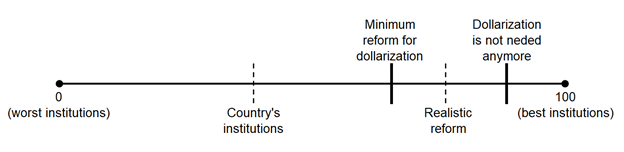
\includegraphics{Figures/Fig_01.png}
    \label{fig:Fig01}
\end{figure}

The institutional robustness of dollarization should not be underestimated. Dollarization in Ecuador survived (1) the left-leaning populist regime of Rafael Correa, (2) a sovereign debt default, (3) the 2008 financial crisis. Arguably, dollarization served as a constrain on populist policies. Absher, Grier, and Grier \parencite*{Absher2020} find that durable left-populist regimes in Latin America produce significant losses in real income. The only exception in their study is Ecuador, which is also the only dollarized country in their study. Using the Economic Freedom of the World Index (EFW) as a proxy of institutional quality, Ecuador ranks 118 out of 162 countries (73 percentile), just below Guyana and above Vietnam \parencite{EFW_2019}. Dollarization survived for two decades in Ecuador, a country where there is still plenty of room of institutional improvement. The low EFW score suggest that dollarization served as an institutional constraint against the populist regime of Rafael Correa. In short, Ecuador did not have to become one of the freest economies in the world to have a durable dollarization.


% ================================================================
% --- SECTION 3: SYNTHETIC CONTROL ANALYSIS
\section{Synthetic Control Analysis}
    \label{sec:SCA}

\subsection{The SCA Method and Donor Pool Selection Criteria}

SCA allows to build a counterfactual non-dollarized Ecuador and compare the evolution of key economic variables such as GDP per capita, TFP, unemployment, and income distribution (GINI coefficient) with real-world dollarized Ecuador. SCA allows to deal with fixed effects interacting with time-varying coefficients when there is only one treated unit (in our case Ecuador). In simpler terms, synthetic Ecuador is a weighted average of countries included in a donor pool. A few requirements are needed for a proper application of the SCA method.

First, the donor pool must include countries that share similar characteristic to the treated unit. SCA prioritizes a representative donor pool over a large-as-possible sample. A larger sample may include non-representative countries that can reduce the efficiency of the estimation or produce overfitting. In SCA, more data is not always better. Second, the treated country must be the only one in the sample being affected by the shock under analysis and the shock must occur at a definite point of time. Ecuador must be the only country going through dollarization. Third, there should be enough observations in the pre-shock period for the SCA to be able to build a credible synthetic Ecuador.

Besides the donor countries, a number of covariates (predictor) variables are chosen as well (see table \ref{table:sources}). The SCA method minimizes the root-mean-squared-prediction-error (MSPE) in the pre-shock period. The values of the covariates is averaged for the pre-shock period. Then SCA minimizes the MSPE during the pre-shock period. To do so, SCA assigns relative weights to each covariate depending how good they are in predicting the outcome variable. This relative weights are captured in a diagonal matrix (the V matrix). The diagonal values of the V matrix are non negative and normalized to one. Therefore, covariates with low explanatory power over the outcome variable have low values in the V matrix. \footnote{More formally, let there be $j = 1,...,J$ countries in the donor pool and $W$ be a vector of non-negative weights assigned to each country $(w_j \geq 0$. Then, SCA estimates $W^*$ such that $W^* = \operatorname{arg\min} (X_1 - X_0W)'V(X_1 - X_0W)$ where $X_1$ contains the covariates from the treated country and $X_0$ contains the covariates it the donor countries. $V$ is a diagonal matrix with non-negative components.}

Our donor pool is limited to Latin America countries to maintain an overall social and economic similarity with Ecuador. The reason to limit our donor pool to Latin America is to avoid the accidental inclusion of a country that not representative enough of Ecuador social and economic characteristics. We also exclude Latin American countries that are dollarized such as Panamá and El Salvador.\footnote{We do include Argentina, which was under a currency board during the 1990s. However, Argentine had an heterodox currency board which allows deviations from its strict (orthodox) adherence \parencite{Hanke2008}.} The donor countries are: (1) Argentina, (2) Bolivia, (3) Brazil, (4) Chile, (5) Colombia, (6) Costa Rica, (7) Mexico, (8) Paraguay, (9) Perú, and (10) Uruguay

\begin{table}[!h]
\begin{center}
\caption{Data source and summary statistics} \label{table:sources}
\begin{tabular}{l r r l} \\ \toprule
  Variable                       & Mean    & Std. Dev.     & Source                     \\ \midrule
  \textbf{Outcomes}              &         &               &                            \\
  GDP per Capita (PPP, 2017)     & \$9,188.59 & \$4,558.72 & The Maddison Project       \\
  TFP (PPP adjusted) (\% change) & -0.66   & 2.85          & The Conference Board       \\
  Unemployment rate              & 7.48    & 3.68          & World Bank (WDI)           \\
  GINI coefficient               & 46.10   & 4.38          & World Bank (WDI) and SWIID \\ \midrule
  \textbf{Covariates}            &         &               &                            \\
  Industry (\% of GDP)           & 30.10   & 5.22          & World Bank (WDI)           \\
  Manufacturing (\% of GDP)      & 17.12   & 4.69          & World Bank (WDI)           \\
  Investment (\% of GDP)         & 18.69   & 4.36          & World Bank (WDI)           \\
  Trade openness                 & 48.08   & 20.85         & World Bank (WDI)           \\
  FDI (\% of GDP)                & 2.57    & 2.35          & World Bank (WDI)           \\
  Labor compensation (\% of GDP) & 48.80   & 6.69          & Penn World Table           \\
  Gross capital formation        & 18.68   & 4.37          & Penn World Table           \\
  Human Capital Index            & 2.39    & 0.33          & World Bank (WDI)           \\
  Urban population (\% of total) & 72.19   & 13.71         & World Bank (WDI)           \\
  \bottomrule 
\end{tabular}
\singlespacing \footnotesize \raggedright
TFP: Total factor productivity; FDI: Foreign direct investment; Gross capital formation is measured as share of GDP in current PPPs
\end{center}
\end{table}

Using all pre-treatment values of the outcome variable to predict its post-treatment values can lead to inaccurate results or bias \parencite{Ashok2015}. Therefore, we offer for two models for each SCA estimation. Besides the chosen covariates, SCA model 1 also uses a few selected values of the outcome variable from the pre-treatment period. SCA model 2 uses only covariates in the pre-treatment period. We use this approach for all SCA estimations below. Table \ref{table:countries} shows the country weight for each outcome variable and for each SCA model.

\begin{table}[!htbp]
\begin{center}
\caption{Country weights per outcome variable and SCA model} \label{table:countries}
\begin{tabular}{l c c c c c c c c} \\ \toprule
  & \multicolumn{2}{c}{GDP per capita (PPP)} & \multicolumn{2}{c}{TFP} & \multicolumn{2}{c}{Unemployment} & \multicolumn{2}{c}{GINI}                \\ 
  Country    & SCA 1 & SCA 2 & SCA 1 & SCA 2 & SCA 1 & SCA 2 & SCA 1 & SCA 2 \\ \midrule
  Argentina  &       &       &  35.8 &  11.7 &       &       &       &       \\
  Bolivia    &  64.6 &       &       &   0.4 &   7.9 &       &       &       \\
  Brazil     &       &       &       &   0.2 &  44.3 &  56.1 &       &       \\
  Chile      &       &       &       &   3.8 &       &       &       &  17.1 \\
  Colombia   &       &       &       &   0.4 &  44.9 &       &       &       \\
  Costa Rica &       &       &       &   0.8 &       &       &  18.8 &   6.4 \\
  Mexico     &  35.4 &  20.5 &  21.3 &  70.8 &       &       &   5.0 &       \\
  Paraguay   &       &  72.8 &  41.0 &   9.2 &       &   7.3 &  37.7 &  76.5 \\
  Perú       &       &   6.7 &   1.9 &   0.8 &   3.8 &  36.6 &  38.6 &       \\
  Uruguay    &       &       &       &   2.0 &       &       &       &       \\
  \bottomrule 
\end{tabular}
\end{center}
\end{table}

\subsection{Real GDP per Capita (PPP)}

Our first estimation is real GDP per capita (PPP adjusted).\footnote{It is common in the SCA literature to use PPP adjusted real GDP per capita. See, for instance, Abadie, Diamond, and Hainmuller \parencite*{Abadie2015}, Absher, Grier, and Grier \parencite*{Absher2020}, Cavallo, Noy, and Pantano \parencite*{Cavallo2013}, Campis, Coricelli, and Moretti \parencite*{Campos2019}, and Lawson, Grier, and Absher \parencite*{Lawson2019}.} Consider that dollarization occurs at the same time that price of commodities start to rise in the early 2000s. It is expected, then, to see an upward trend in Ecuador's income per capita with or without dollarization. This situation with a coincidence in when dollarization takes place and when commodity prices start to rise exemplifies that the ideal conterfactual is not what happens to Ecuador's economy before and after dollarization, but how does dollarized Ecuador compares had dollarization not happened. 

Tables \ref{table:GDP_balance} shows the predictor balance, V matrix values, and RMSPE for both SCA models. With the given sample, two or three countries are needed to minimize the RMSPE of synthetic Ecuador. The tables show that the model that includes two observations of the outcome variable has a lower RMSPE, but the outcome values carry most of the weight as explanatory values.

\begin{table}[!h]
\begin{center}
\caption{SCA for GDP per Capita (PPP), predictor balance, V matrix, and RMSPE} \label{table:GDP_balance}
\begin{tabular}{l r r r r r r}     \\ \toprule
  Variable                    &    Ecuador &  Synthetic 1 & V matrix 1 & Synthetic 2 & V matrix 2 \\ \midrule 
  Industry (\% GDP)           &      28.41 &        29.79 &     0.0163 &       28.88 &     0.4592 \\
  Manufacturing (\% GDP)      &      21.35 &        16.65 &     0.0131 &       15.80 &     0.0064 \\
  Investment (\% GDP)         &      21.15 &        14.30 &     0.0005 &       19.87 &     0.5262 \\
  Unemployment rate           &       8.53 &         7.39 &     0.0001 &        5.47 &     0.0083 \\ \midrule
  GDP per capita (PPP) (1981) & \$5,831.00 &   \$5,627.20 &     0.6631 &             &            \\
  GDP per capita (PPP) (1999) & \$4,797.00 &   \$5,621.58 &     0.3070 &             &            \\ \midrule
  RMSPE                       &            &       315.62 &            &      375.11 &            \\
  \bottomrule 
\end{tabular}
\end{center}
\end{table}

Figure \ref{fig:SCA_GDP} depicts dollarized Ecuador along both SCA estimations. As expected, we see the three lines starting an upward trend at the same time the price of commodities start to rise. However, the GDP per capita (adjusted for cost of living) outperforms both SCA estimations; real income of Ecuador grew more than it would have absent the dollarization reform. The plot also depicts the impact of the 2008 crisis. Despite being dollarized, Ecuador's real GDP (PPP) remained higher than the non-dollarized counterfactual estimations.

\begin{figure}[!htbp]
    \caption{SCA: Real GDP per capita (PPP)}
    \centering
    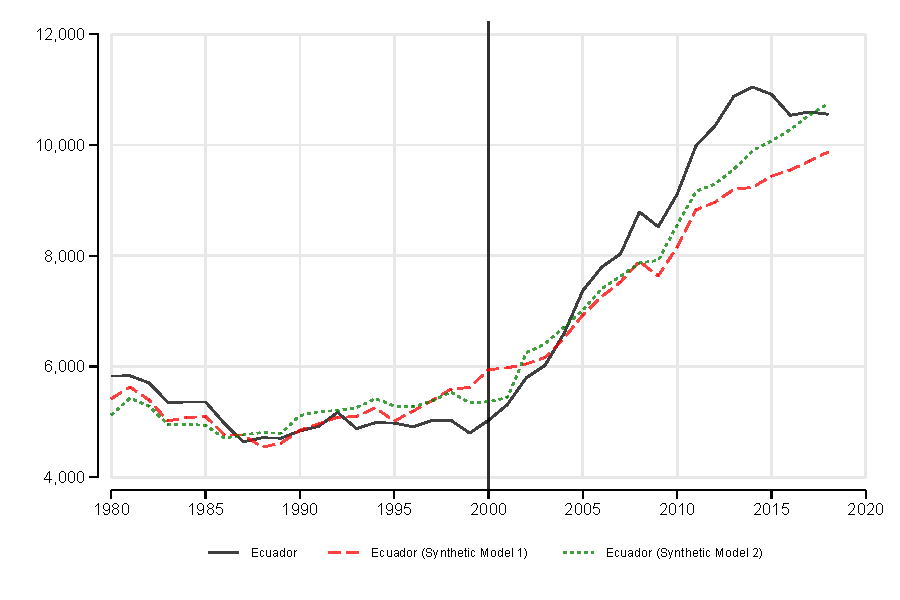
\includegraphics{STATA/Fig_GDP_SCA.pdf}
    \label{fig:SCA_GDP}
\end{figure}

The plot also shows that starting in 2015 Ecuador's real GDP (PPP) falls and then stagnates in 2016. This does not occur in the counterfactual, which may suggest that the issue rests on the use of a foreign currency. However, the reason for this change in trend is a combination of (1) fall in oil prices, (2) increased tax on exports, and (3) the 2016 earthquake. The latter was absent in the donor countries that build the synthetic Ecuador. These new shocks mean that dollarization is not the obvious reason of the change in real income. 

The spread between dollarized Ecuador and its synthetic estimations is economically significant. By 2005, Ecuador is producing a 5-percent higher real income (PPP adjusted), by 2010 Ecuador is producing between 8-percent and 11-percent higher than the synthetic estimations (figure \ref{fig:SCA_gap}). At the peak, dollarization brought between 12-percent and 20-percent of higher PPP adjusted real income. It plausible that monetary stability and credible reform brought more benefits than being undefended of foreign shocks (recall that Ecuador still has a liquidity fund at its disposal).

\begin{figure}[!htbp]
    \caption{SCA: Real GDP per capita (PPP) synthetic gap}
    \centering
    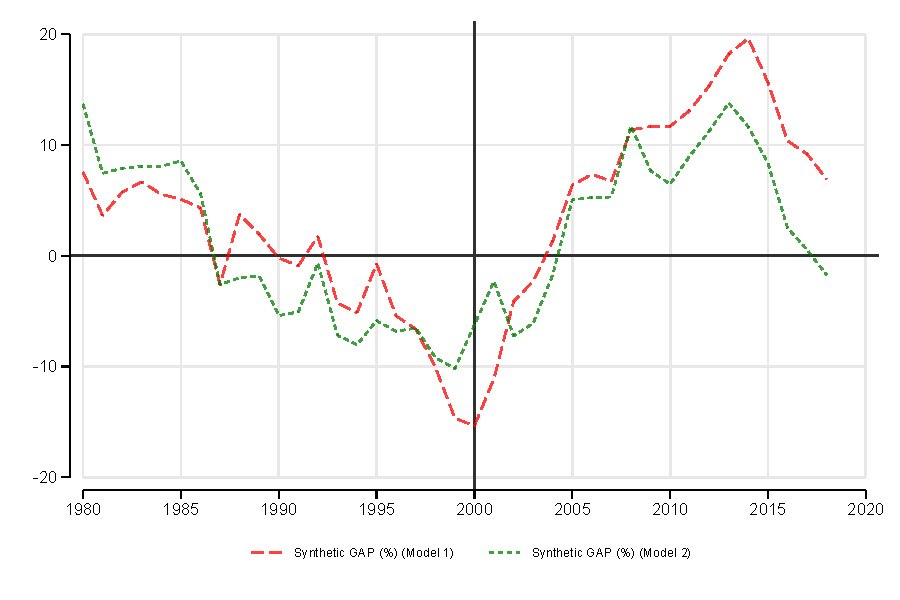
\includegraphics{STATA/Fig_GDP_GAP.pdf}
    \label{fig:SCA_gap}
\end{figure}

\subsection{Total Factor Productivity}

Similar to GDP, we use PPP adjusted growth rates of GDP. While TFP growth rates are small in magnitude, they do depict opposite signs. Ecuador has a 0.14-percent average annual growth rate of TFP, while synthetic estimations result in  negative 0.02-percent and negative 0.35-percent annual average growth for both model estimations respectively. It is likely that Ecuador needs more regulatory reforms in order to benefit from larger TFP growth rates. Recall that Ecuador ranks low in the EFW index and that dollarization is not a sufficient, even if necessary, reform.

We show first the predictor balance and V matrix for each SCA model. Even though values from the outcome variable have vey low V matrix values, its RMSPE is lower than the model without using outcome values as predictors. Figure \ref{fig:SCA:TFP} depicts the SCA results. Consider three points in the plot. The first one is the quicker recovery of TFP growth rates immediately after the dollarization reform which does not occur in either synthetic estimation. The second is the nominal shock of the 2008 crisis, Ecuador's TFP falls less than the non-dollarized counterfactuals. The third one is, again, the slow down of the economy starting in 2014. As discussed in the previous section, this is due to a new set of shocks affecting Ecuador's economy.

\begin{table}[!htbp]
\begin{center}
\caption{SCA for TFP (PPP and in real terms), predictor balance, V matrix, and RMSPE} \label{table:TFP_balance}
\begin{tabular}{l r r r r r r}     \\ \toprule
  Variable                    &    Ecuador &  Synthetic 1 & V matrix 1 & Synthetic 2 & V matrix 2 \\ \midrule 
  Investment (\% GDP)         &     19.31  &       18.30  &       0.00 &      19.33  &       0.28 \\
  Trade openness              &     44.93  &       57.24  &       0.00 &      44.99  &       0.21 \\ 
  FDI (\% GDP)                &      2.06  &        2.06  &      ~1.00 &       2.06  &       0.23 \\
  HCI                         &      2.32  &        2.32  &       0.00 &       2.32  &       0.28 \\
  Labor compensation (\% GDP) &     37.00  &       44.86  &      ~0.00 &      42.28  &       0.00 \\ \midrule
  TFP (1995)                  &     -0.93  &       -1.22  &      ~0.00 &             &            \\
  TFP (1999)                  &     -3.23  &       -3.52  &       0.00 &             &            \\ \midrule
  RMSPE                       &            &        1.10  &            &       2.15  &            \\
  \bottomrule 
\end{tabular}
\end{center}
\end{table}

\begin{figure}[!htbp]
    \caption{SCA: TFP (constant prices and PPP adjusted)}
    \centering
    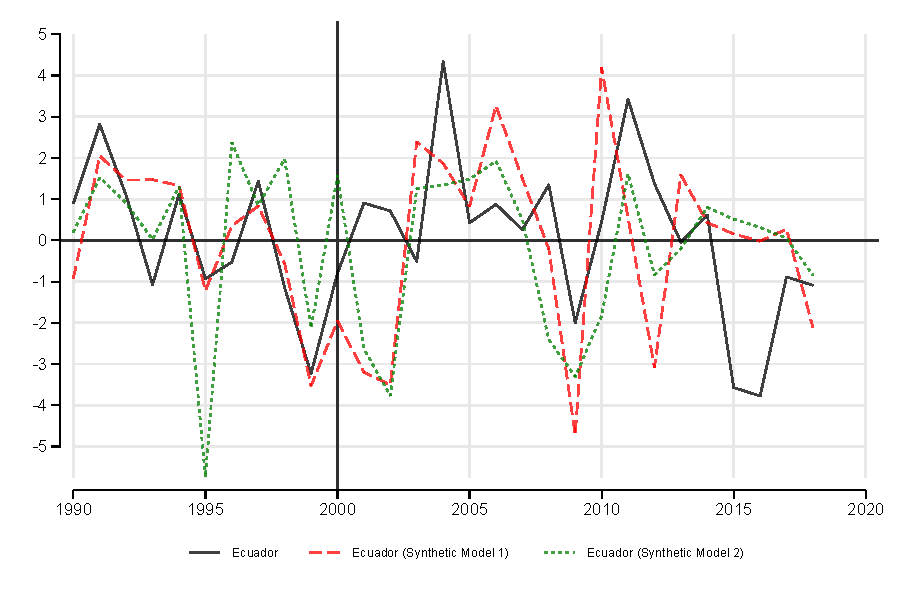
\includegraphics{STATA/Fig_TFP3_SCA.pdf}
    \label{fig:SCA_TFP}
\end{figure}

\subsection{Unemployment}

\subsection{GINI coefficient}

% ================================================================
% --- SECTION 4: CONCLUSIONS


% ================================================================
% --- SECTION 5: REFERENCES
\newpage
\singlespacing
\printbibliography


% ================================================================
% --- THE END
\end{document}
